\chapter{Arhitektura i dizajn sustava}
      
      {Arhitektura sustava naše aplikacije implementirana je u arhitekturi klijent-poslužitelj.}
       
      {Na klijentskoj strani koristili smo programski jezik \textit{JavaScript}, radni okvir \textit{React} i biblioteku komponenata \textit{Material UI} u uređivaču \textit{Visual Studio Code}.}
      
      {Na poslužiteljskoj strani koristili smo programski jezik \textit{Java} i radni okvir \textit{Spring Boot} u uređivaču \textit{IntelliJ IDEA}. Poslužiteljska strana organizirana je u tri sloja. To su nadglednik (controller), usluga (service) i repozitorij (repository). Nadglednik povezuje korisničku stranu s poslužiteljskom stranom. Sloj usluga ostvaruje temeljnu funkcionalnost web aplikacije i definira jednu ili više usluga web aplikacije. Repozitorij osigurava pristup podacima.}
      	
      {Podatke smo spremali u relacijsku bazu podataka \textit{PostgreSql} koristeći \textit{Java Persistence API}.} 
      
      
      \begin{figure}[H]
      	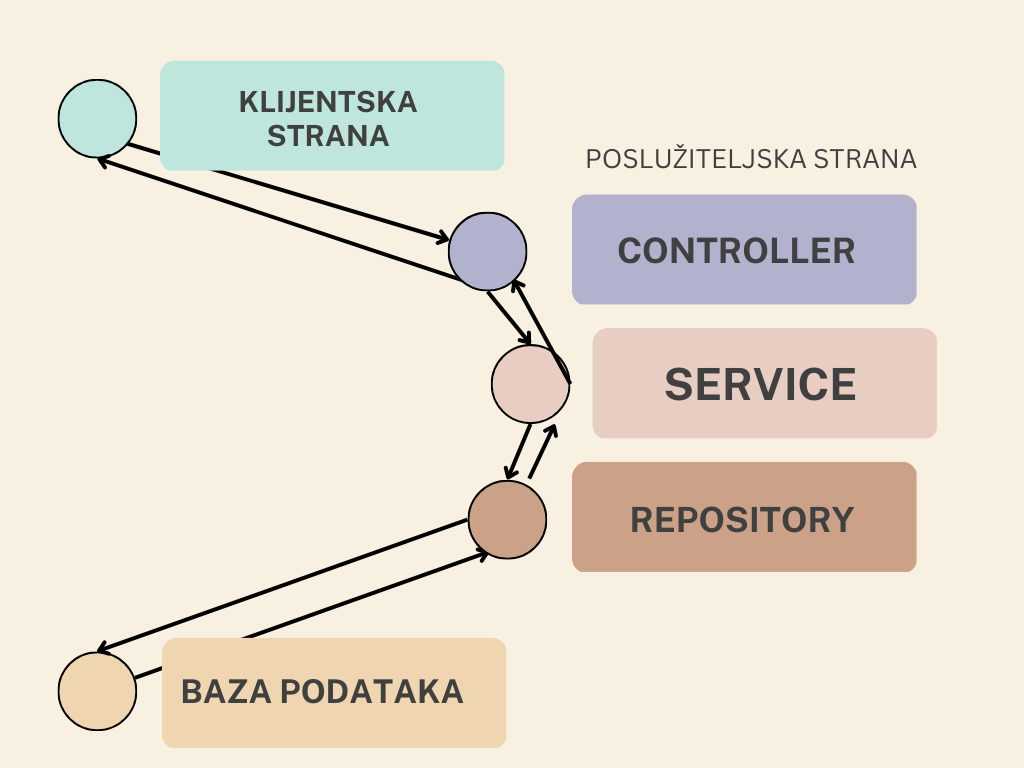
\includegraphics[scale=0.3]{slike/povezanostslojeva.PNG} %veličina slike u odnosu na originalnu datoteku i pozicija slike
      	\centering
      	\caption{Povezanost slojeva u radnom okviru Spring}
      	\label{fig:povezanostslojeva.png}
      \end{figure}
  
      {Osim toga postoji i razrađeni model podataka domene (domenski
      	objekti) kojeg koriste svi slojevi po potrebi. Razredi koji su sadržani u modelu domene imaju oznaku @Entity i sadrže podatke koji se
      	postavljaju i čitaju putem metoda get i set. Nadglednik koristi domenske objekte za automatsko postavljanje vrijednosti objekata iz tijela
      	zahtjeva (@RequestBody) od klijentske strane, sloj usluge korisit ih za ostvarenje odgovarajuće funkcionalnosti aplikacije, a repozitorij za automatskopreslikavanje objekta u relaciju u bazi podataka i obratno.}
      
      



				
		\section{Baza podataka}
		
		 {U implementaciji naše web aplikacije koristimo relacijsku bazu podataka. Objekti u relacijskoj bazi podataka su relacije, tj. dvodimenzionalne tablice koje su definirane imenom, a atributi su imenovani stupci relacije. Glavna zadaća baze podataka je pohrana, izmjena i dohvat podataka za daljnju obradu. Baza podataka ove aplikacije sastoji se od sljedećih entiteta: }
		  \begin{packed_item}
		  	\item {User}
		  	\item {Updates}
		  	\item {TrainingSession}
		  	\item {TrainingType}
		  	\item {Exercise}
		  	\item {Goal}
		  \end{packed_item}
		
			\subsection{Opis tablica}
			

				{Entitet \textbf {User} sadrži sve podatke o korisniku aplikacije.Sadrži atribute korisničko ime, ime korisnika, prezime, email adresu, lozinku, ulogu koju korisnik ima, prvi i drugi cilj, preostali broj termina treninga koje korisnik ima pravo rezervirati ovaj mjesec i novi cilj korisnika. Ovaj entitet u vezi je \textit{One-to-One} s entitetom \textit{Updates} preko atributa username i u vezi je s \textit{Many-to-One} s \textit{TrainingSession} preko atributa username.
				
				\begin{longtblr}[
					label=none,
					entry=none
					]{
						width = \textwidth,
						colspec={|X[11,l]|X[6, l]|X[20, l]|}, 
						rowhead = 1,
						cell{1}{1} = {c=3}{c},
					}
					\hline 
					\textbf{User} & & 	 \\ \hline[3pt]
					\SetCell{LightGreen}username & VARCHAR	&  	jedinstveno korisničko ime	\\ \hline
					firstName	& VARCHAR &   ime korisnika	\\ \hline 
					lastName & VARCHAR & prezime korisnika  \\ \hline 
					email & VARCHAR	&  	e-mail korisnika	\\ \hline 
					password & VARCHAR	&  	lozinka korisnika	\\ \hline
					role & VARCHAR	&  	uloga korisnika	\\ \hline
					goal1 & VARCHAR	&  	prvi cilj korisnika	\\ \hline 
					goal2 & VARCHAR	&  	drugi cilj korisnika	\\ \hline 
					remainingTrainingSessions & INT	&  	preostali termini korisnika \\ \hline
					newGoal & INT	&   novi cilj	\\ \hline 	 
				\end{longtblr}
			
			{Entitet \textbf{Updates} identifikacijski je slabi entitet koji ovisi o entitetu \textit{User}. Sadrži podatke o zadnjem ažuriranju preostalih termina korisnika i posljednjoj promjeni ciljeva korisnika. Sadrži atribute korisničko ime, oznaku kada je ažuriran fond sati i oznaku kada je omogućena posljednja promjena cilja. Ovaj entitet u vezi je \textit{One-to-One} s entitetom \textit{User} preko atributa username.
			
			\begin{longtblr}[
				label=none,
				entry=none
				]{
					width = \textwidth,
					colspec={|X[11,l]|X[6, l]|X[20, l]|}, 
					rowhead = 1,
					cell{1}{1} = {c=3}{c},
				}
				\hline 
				\textbf{Updates} & & \\ \hline[3pt]
				\SetCell{LightGreen} username & VARCHAR & jedinstveno korisničko ime	\\ \hline
				sessionsUpdate & TIMESTAMP & oznaka kad je ažuriran fond sati  \\ \hline
				goalsUpdate & TIMESTAMP & oznaka kad je omogućena posljednja promjena cilja  \\ \hline  
					 
			\end{longtblr}
		
		     {Entitet \textbf{TrainingSession} sadrži podatke o terminima treninga. Sadrži atribute identifikator termina treninga, početno vrijeme treninga, vrijeme kad završava trening, korisničko ime i identifikator vrste treninga. Ovaj entitet u vezi je \textit{One-to-Many} s entitetom \textit{User} preko atributa username., u vezi \textit{One-to-One} s entitetom \textit{TrainingType} preko atributa trainingTypeId  te u vezi \textit{One-to-One} s entitetom \textit{Exercise} preko atributa exerciseId i trainingSessionId te se na vezi nalazi atribut TrainingExerciseId. 
			
			\begin{longtblr}[
				label=none,
				entry=none
				]{
					width = \textwidth,
					colspec={|X[11,l]|X[6, l]|X[20, l]|}, 
					rowhead = 1,
					cell{1}{1} = {c=3}{c},
				}
				\hline \textbf{TrainingSession} & & \\ \hline[3pt]
				\SetCell{LightGreen}trainingSessionId & INT	&  	jedinstveni identifikator termina treninga	\\ \hline
				startDateTime	& TIMESTAMP &   početak treninga	\\ \hline 
				endDateTime & TIMESTAMP & kraj treninga  \\ \hline 
				\SetCell{LightBlue} username & VARCHAR & jedinstveno korisničko ime 	\\ \hline
				\SetCell{LightBlue} trainingTypeId & INT & jedinstveni identifikator treninga	\\ \hline
			\end{longtblr}
		
		{Entitet \textbf{TrainingType} sadrži podatke o vrsti treninga. Sadrži atribute jedinstveni identifikator treninga i naziv vrste treninga. Ovaj entitet u vezi je \textit{One-to-One} s entitetom \textit{User} preko atributa username.
		
		\begin{longtblr}[
			label=none,
			entry=none
			]{
				width = \textwidth,
				colspec={|X[11,l]|X[6, l]|X[20, l]|}, 
				rowhead = 1,
				cell{1}{1} = {c=3}{c},
			}
			\hline \textbf{TrainingType} & &	 \\ \hline[3pt]
			\SetCell{LightGreen}trainingTypeId & INT	&  	jedinstveni identifikator treninga	\\ \hline
			trainingType	& VARCHAR &   vrsta treninga	\\ \hline 
		\end{longtblr} 
	
	    {Entitet \textbf{Exercise} sadrži podatke o vježbama. Sadrži atribute jedinstveni identifikator vježbe i naziv vježbe. Ovaj entitet u vezi je \textit{One-to-One} s entitetom \textit{TrainingSession} preko atributa trainingSessionId i exerciseId te se na vezi nalazi atribut trainingExerciseId.
	     
	     \begin{longtblr}[
	     	label=none,
	     	entry=none
	     	]{
	     		width = \textwidth,
	     		colspec={|X[11,l]|X[6, l]|X[20, l]|}, 
	     		rowhead = 1,
	     		cell{1}{1} = {c=3}{c},
	     	}
	     	\hline \textbf{Exercise} & &	 \\ \hline[3pt]
	     	\SetCell{LightGreen}exerciseId & INT	&  	jedinstveni identifikator vježbe	\\ \hline
	     	exercise	& VARCHAR &   vježba	\\ \hline 
	     \end{longtblr}
     
     \begin{longtblr}[
     	label=none,
     	entry=none
     	]{
     		width = \textwidth,
     		colspec={|X[11,l]|X[6, l]|X[20, l]|}, 
     		rowhead = 1,
     		cell{1}{1} = {c=3}{c},
     	}
     	\hline
     	\textbf{TrainingExercise} & &	 \\ \hline[3pt]
     	\SetCell{LightGreen}trainingExerciseId & INT	&  	jedinstveni identifikator vježbe treninga	\\ \hline
     	\SetCell{LightBlue}exerciseId & INT	&  	jedinstveni identifikator vježbe	\\ \hline
     	\SetCell{LightBlue}trainingSessionId & INT	&  	jedinstveni identifikator termina treninga	\\ \hline
     	
     \end{longtblr}
 
        {Entitet \textbf{Goal} sadrži podatke o ciljevima korisnika. Sadrži atribute jedinstveni identifikator cilja i naziv cilja.
     
         \begin{longtblr}[
         	label=none,
         	entry=none
         	]{
         		width = \textwidth,
         		colspec={|X[11,l]|X[6, l]|X[20, l]|}, 
         		rowhead = 1,
         		cell{1}{1} = {c=3}{c},
         	}
         	\hline 
         	\textbf{Goal} & &	 \\ \hline[3pt]
         	\SetCell{LightGreen}goalId & INT	&  	jedinstveni identifikator cilja	\\ \hline
         	goal	& VARCHAR &   cilj	\\ \hline 
         \end{longtblr}
     
				
			
			\subsection{Dijagram baze podataka}
			
			\begin{figure}[H]
				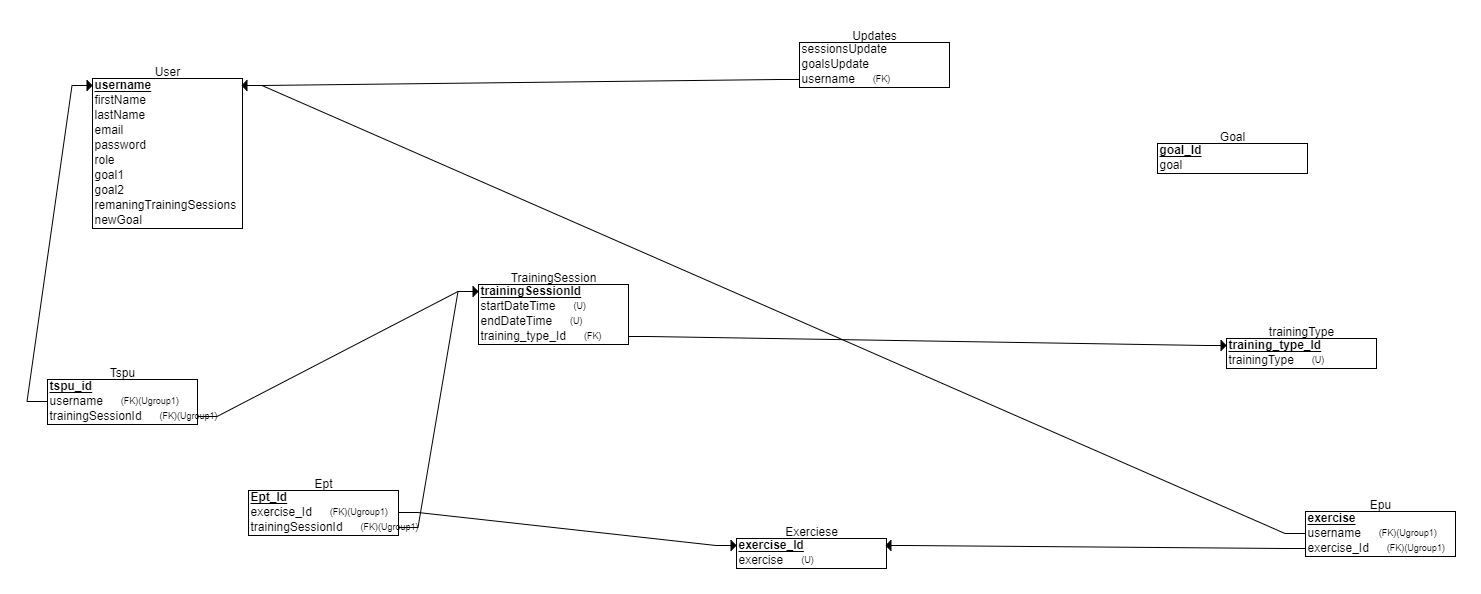
\includegraphics[scale=0.3]{dijagrami/image (8).png} %veličina slike u odnosu na originalnu datoteku i pozicija slike
				\centering
				\caption{dijagram baze podataka}
				\label{fig:diagramRAZ2}
			\end{figure}
			
			
		\section{Dijagram razreda}
		
			{Na sljedećij nekoliko fotografija(4.3, 4.4, 4.5, 4.6 te 4.7) prikazani su razredi backenda koji pripadaju spring arhitektur točnije troslojnom modelu. Konkretno na fotografiji 4.3 prikazani su controller razredi, na fotografiji 4.4 razredi modela, na fotografiji 4.5 razredi repozitorija, na fotografiji 4.6 razredi pripadnih entiteta te na fotografiji 4.7 razredi servisa .}\\
			
			{Nadalje dijagrami su organizirani tako da zrcale  kompontente backend infrastrukture kako bih dijagrami bili pregledniji te logički smisleni.}\\
			
			
			\begin{figure}[H]
				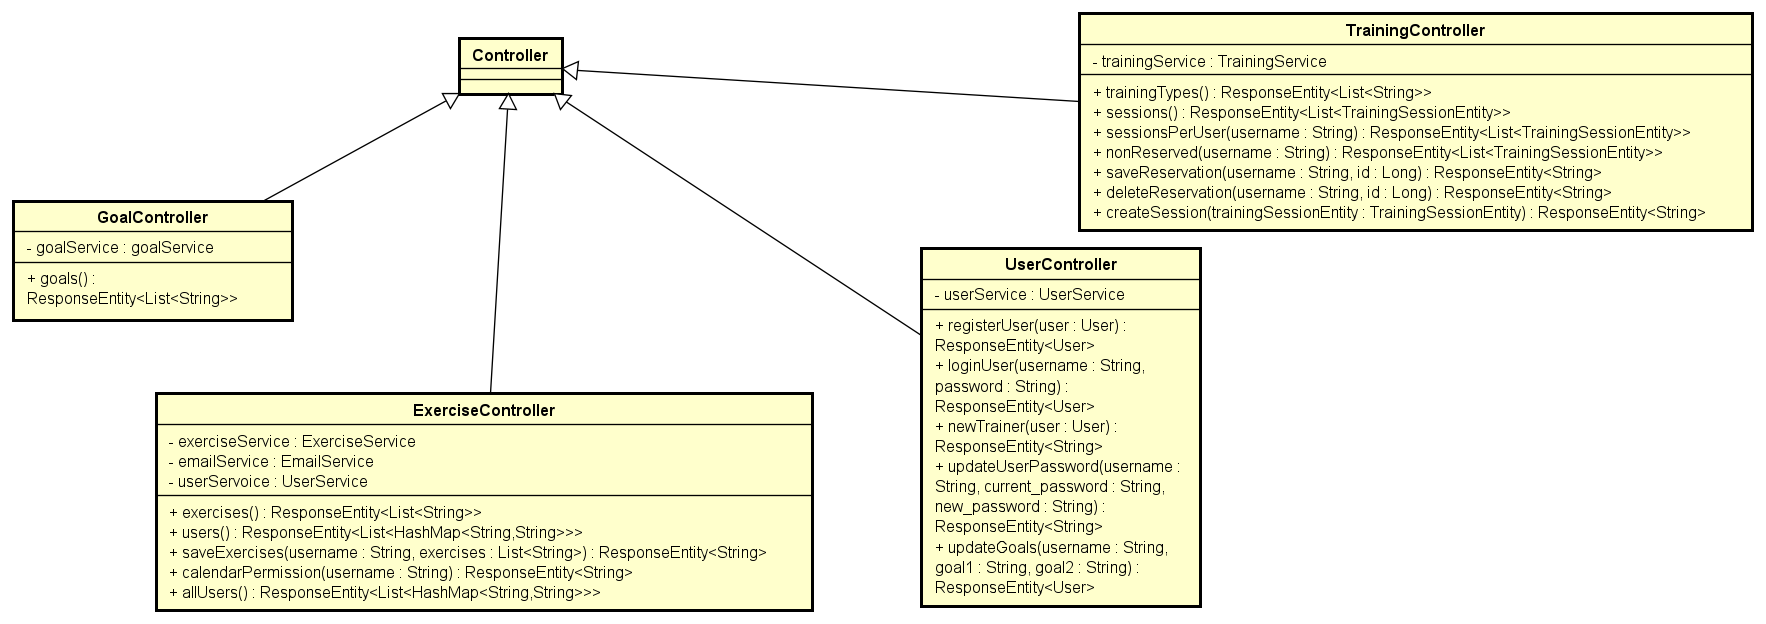
\includegraphics[scale=0.3]{dijagrami/ControllerFinalVersion.png} %veličina slike u odnosu na originalnu datoteku i pozicija slike
				\centering
				\caption{dijagram razreda - Dijagram kontrolera}
				\label{fig:diagramRAZ1}
			\end{figure}
		
			
			
			\begin{figure}[H]
				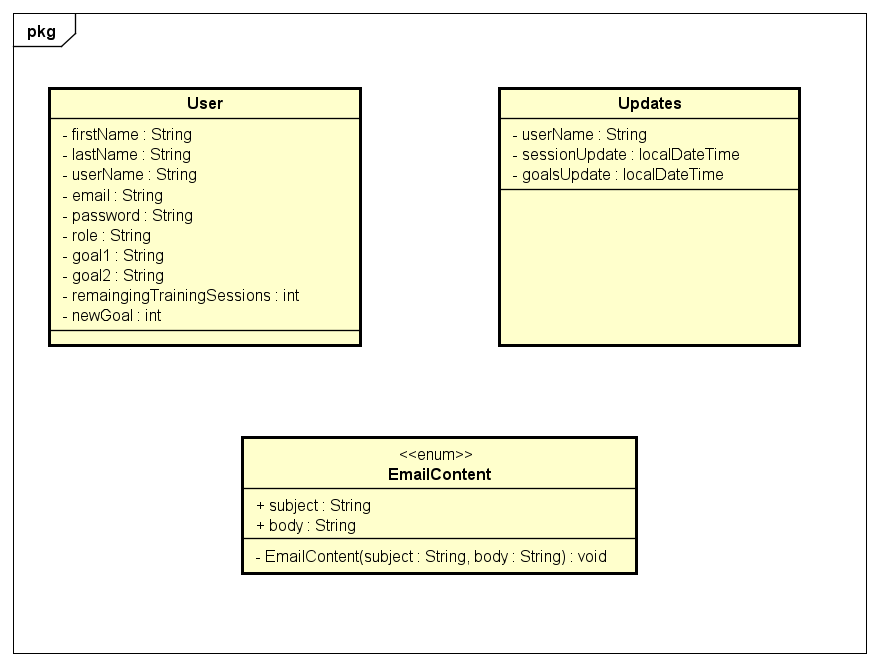
\includegraphics[scale=0.6]{dijagrami/ModelsFinalVersion.png} %veličina slike u odnosu na originalnu datoteku i pozicija slike
				\centering
				\caption{dijagram razreda - Dijagram modela}
				\label{fig:diagramRAZ2}
			\end{figure}
			
			{Na fotografiji 4.4 prikazan je dijagram razreda modela koji preslikavaju entitete i atribute istih na temelju modela baze podataka. }
		
			\begin{figure}[H]
				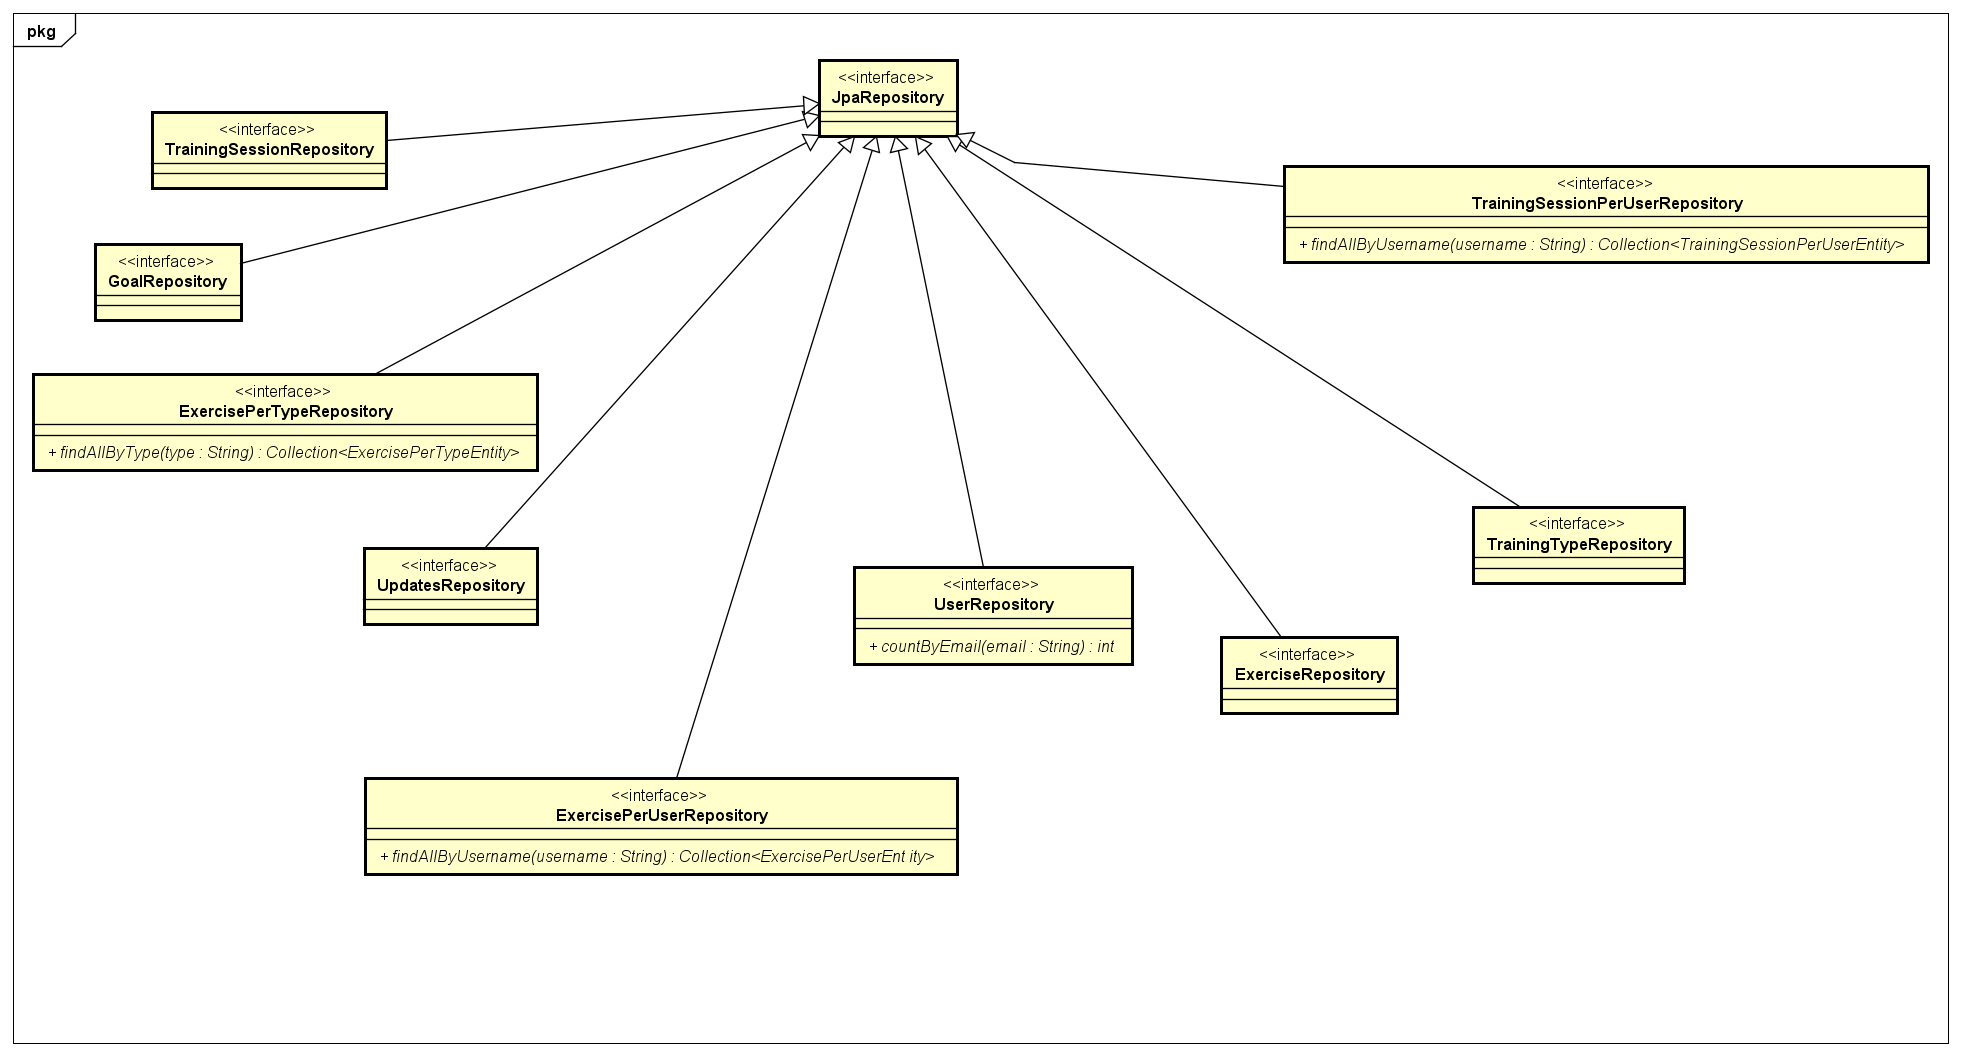
\includegraphics[scale=0.3]{dijagrami/RepositoryFinalVersion.png} %veličina slike u odnosu na originalnu datoteku i pozicija slike
				\centering
				\caption{dijagram razreda - Dijagram repozitorija}
				\label{fig:diagramRAZ3}
			\end{figure}
		
		
			\begin{figure}[H]
				\includegraphics[scale=0.3]{dijagrami/EntitiesFinalVersion.png} %veličina slike u odnosu na originalnu datoteku i pozicija slike
				\centering
				\caption{dijagram razreda - dijagram entiteta}
				\label{fig:diagramRAZ4}
			\end{figure}
		
			\begin{figure}[H]
				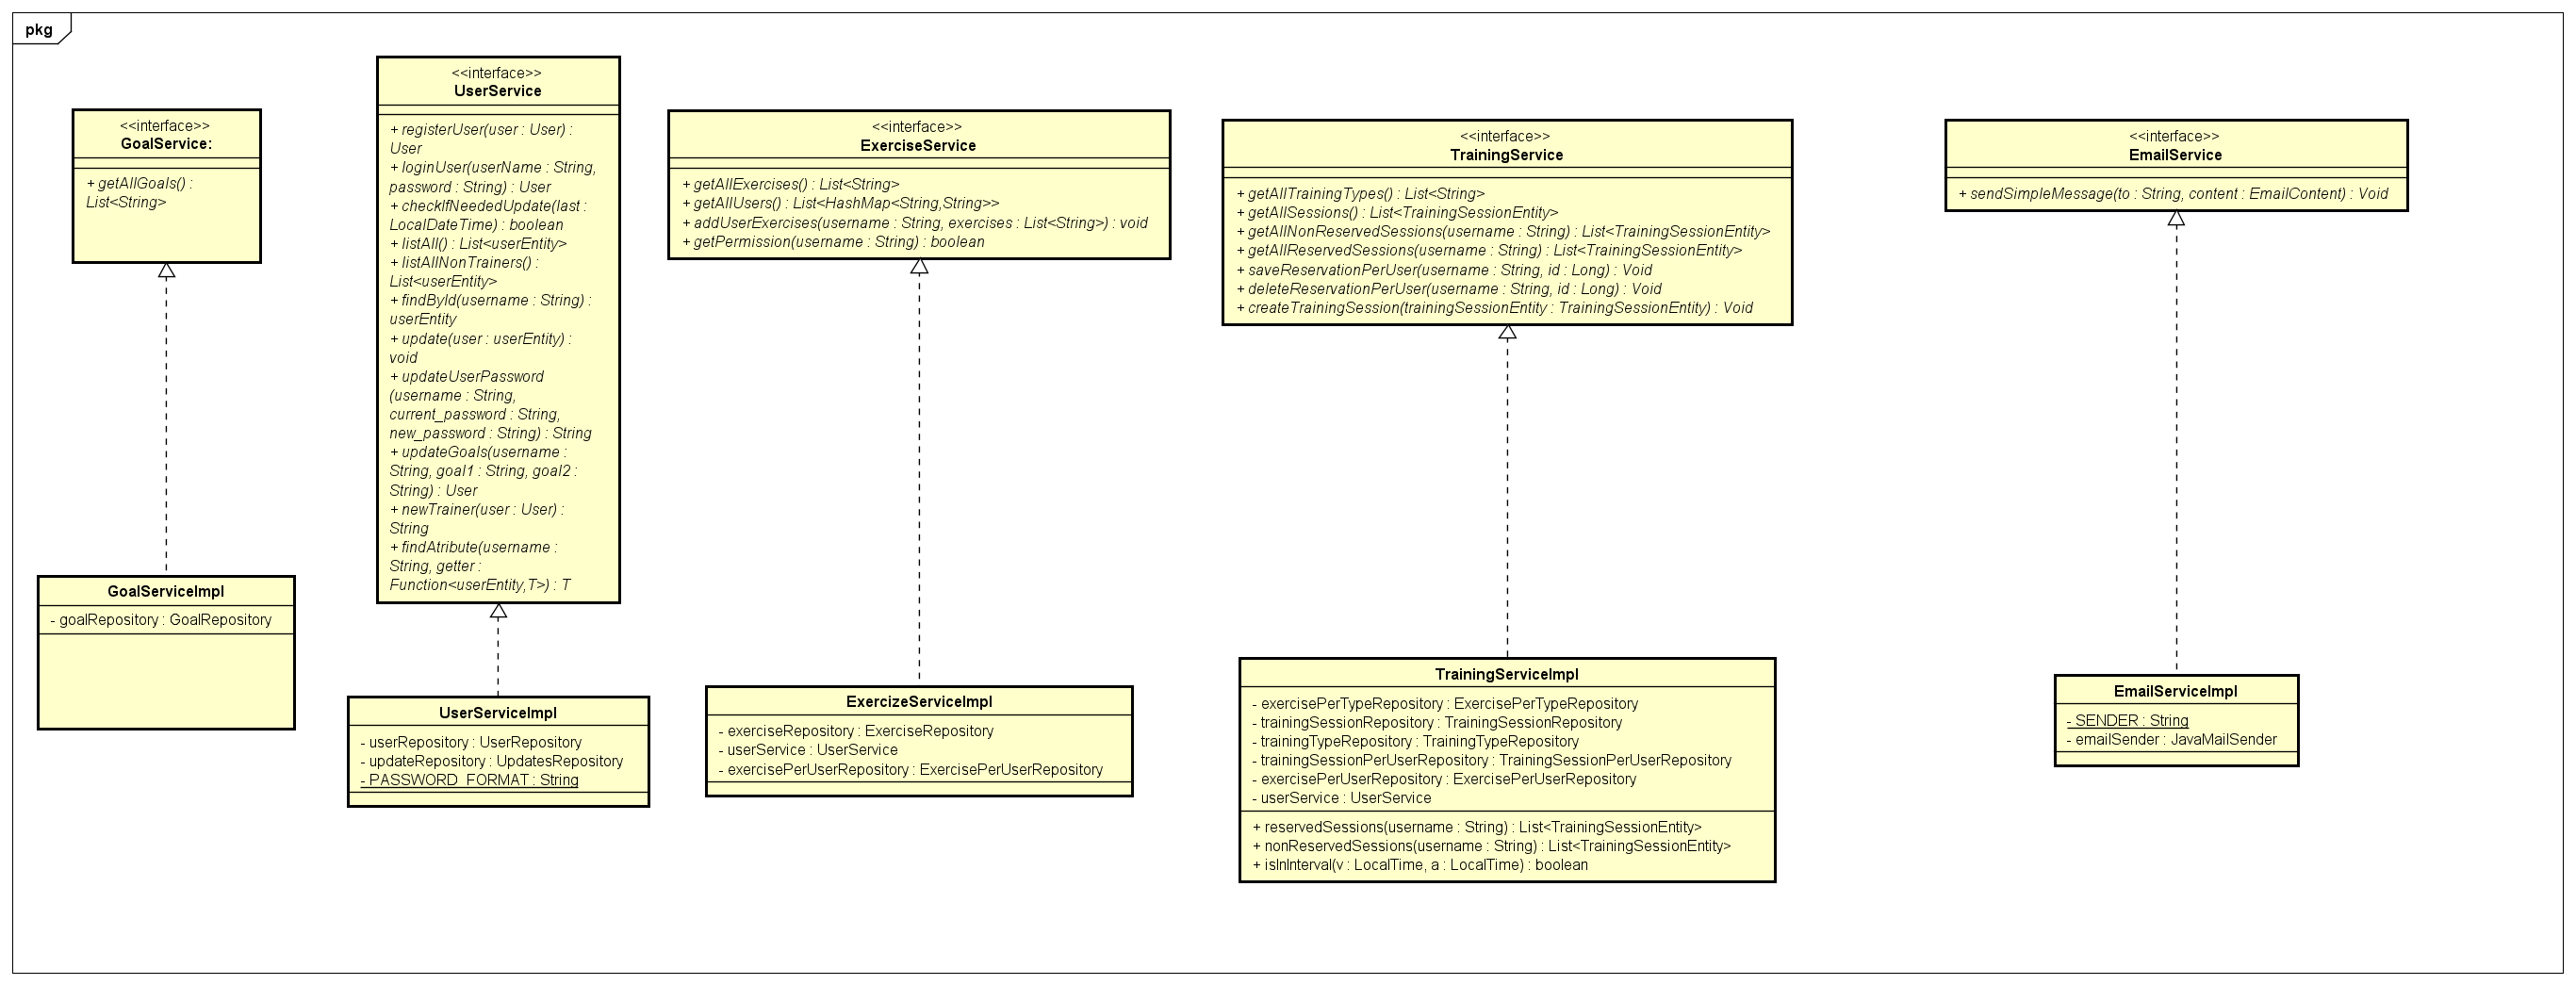
\includegraphics[scale=0.2]{dijagrami/servicesFinalVersion.png} %veličina slike u odnosu na originalnu datoteku i pozicija slike
				\centering
				\caption{dijagram razreda - dijagram servisa}
				\label{fig:diagramRAZ5}
			\end{figure}

		
		
			\textbf{\textit{dio 2. revizije}}\\			
			
			{Prilikom druge predaje projekta dijagram razreda i opisi moraju odgovarati stvarnom stanju implementacije}
			
			
			
			\eject
		
		\section{Dijagram stanja}
			
			{Dijagram stanja opisuje dinamičko ponašanje dijela sustava u vremenu, prikazuje stanja objekta te prijelaze iz jednog stanja u drugo temeljene na događajima. Na slici \ref {fig:dijagramstanja} prikazan je dijagram stanja za registriranog korisnika treninga. Nakon prijave, korisniku se prikazuje njegov personalizirani kalendar. Odabirom određenog termina prikazuju mu se podatci o treningu, to jest od kojih se vježbi sastoji i koliko traje. Ako korisnik ima preostalih sati te određeni termin nije popunjen, korisniku je omogućen gumb "Reserve training session" te klikom na gumb rezervira trening. U slučaju da je korisnikov fond sati nula i/ili da je termin popunjen korisniku je gumb onemogućen te klikom na njega pojavljuje mu se pop-up poruka da ne može rezervirati trening. Također, u zaglavlju stranice korisnik može odabrati neku od ponuđenih mogućnosti. Klikom na "Home page", korisniku se prikazuje naslovna stranica, a klikom na "Profile page" prikazuje mu se stranica s osobni podatcima. Tamo se nalaze osobni podatci korisnika te njegov odabrani cilj. Ukoliko je početak mjeseca, utoliko je korisniku omogućen padajući izbornik za promjenu cilja. Takoeđer, klikom na gumb za uređivanje profila korisniku je omogućena izmjena podataka te mu je prikazan gumb za brisanje korisničkog profila. }
			
			\begin{figure}[H]
				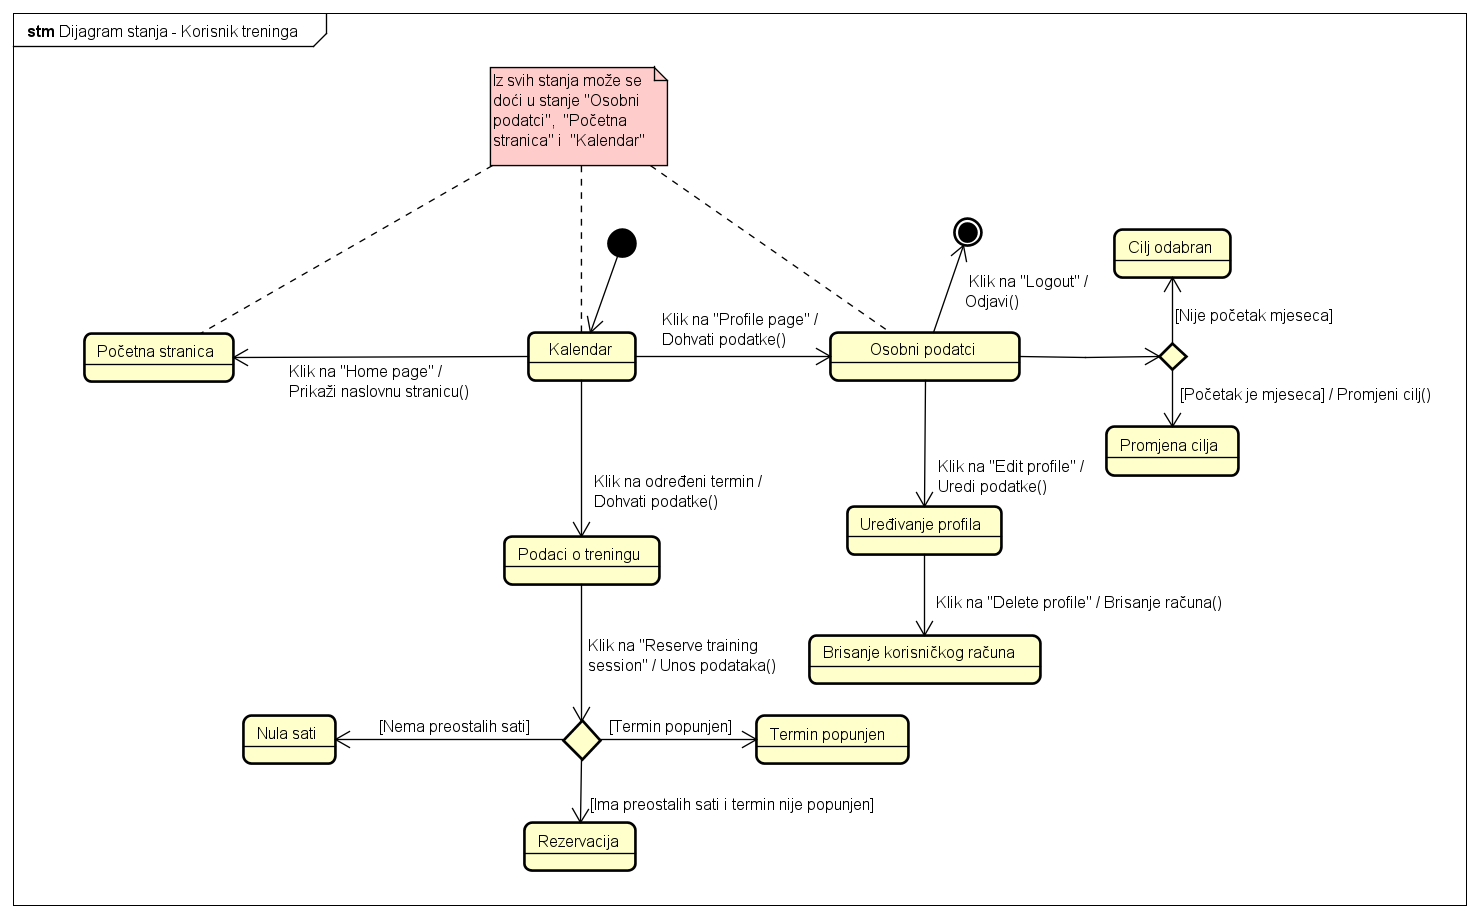
\includegraphics[scale=0.4]{dijagrami/Dijagram stanja - Korisnik treninga.png} %veličina slike u odnosu na originalnu datoteku i pozicija slike
				\centering
				\caption{Dijagram stanja - Korisnik treninga}
				\label{fig:dijagramstanja}
			\end{figure}
			\eject 
		
		\section{Dijagram aktivnosti}
			 
			 {Dijagrami aktivnosti primjenjuju se za modeliranje poslovnih procesa i upravljačkog i podatkovnog toka. Na slici \ref{fig:dijagramaktivnosti} prikazan je proces rezervacije treninga. Korisnik se prijavi u sustav, prikaže mu se personalizirani kalendar i odabire termin treninga za koji želi napraviti rezervaciju. U slučaju da korisnik ima preostaloh sati te da termin nije popunjen, rezervacija se sprema te se prikazuje potvrda rezervacije. Ako je korisnikov fond sati nula ili je termin popunjen, korisniku je onemogućen gumb za rezervaciju te se klikom na njega prikazuje pop-up poruka da ne može rezervirati trening.}
			 
			 \begin{figure}[H]
			 	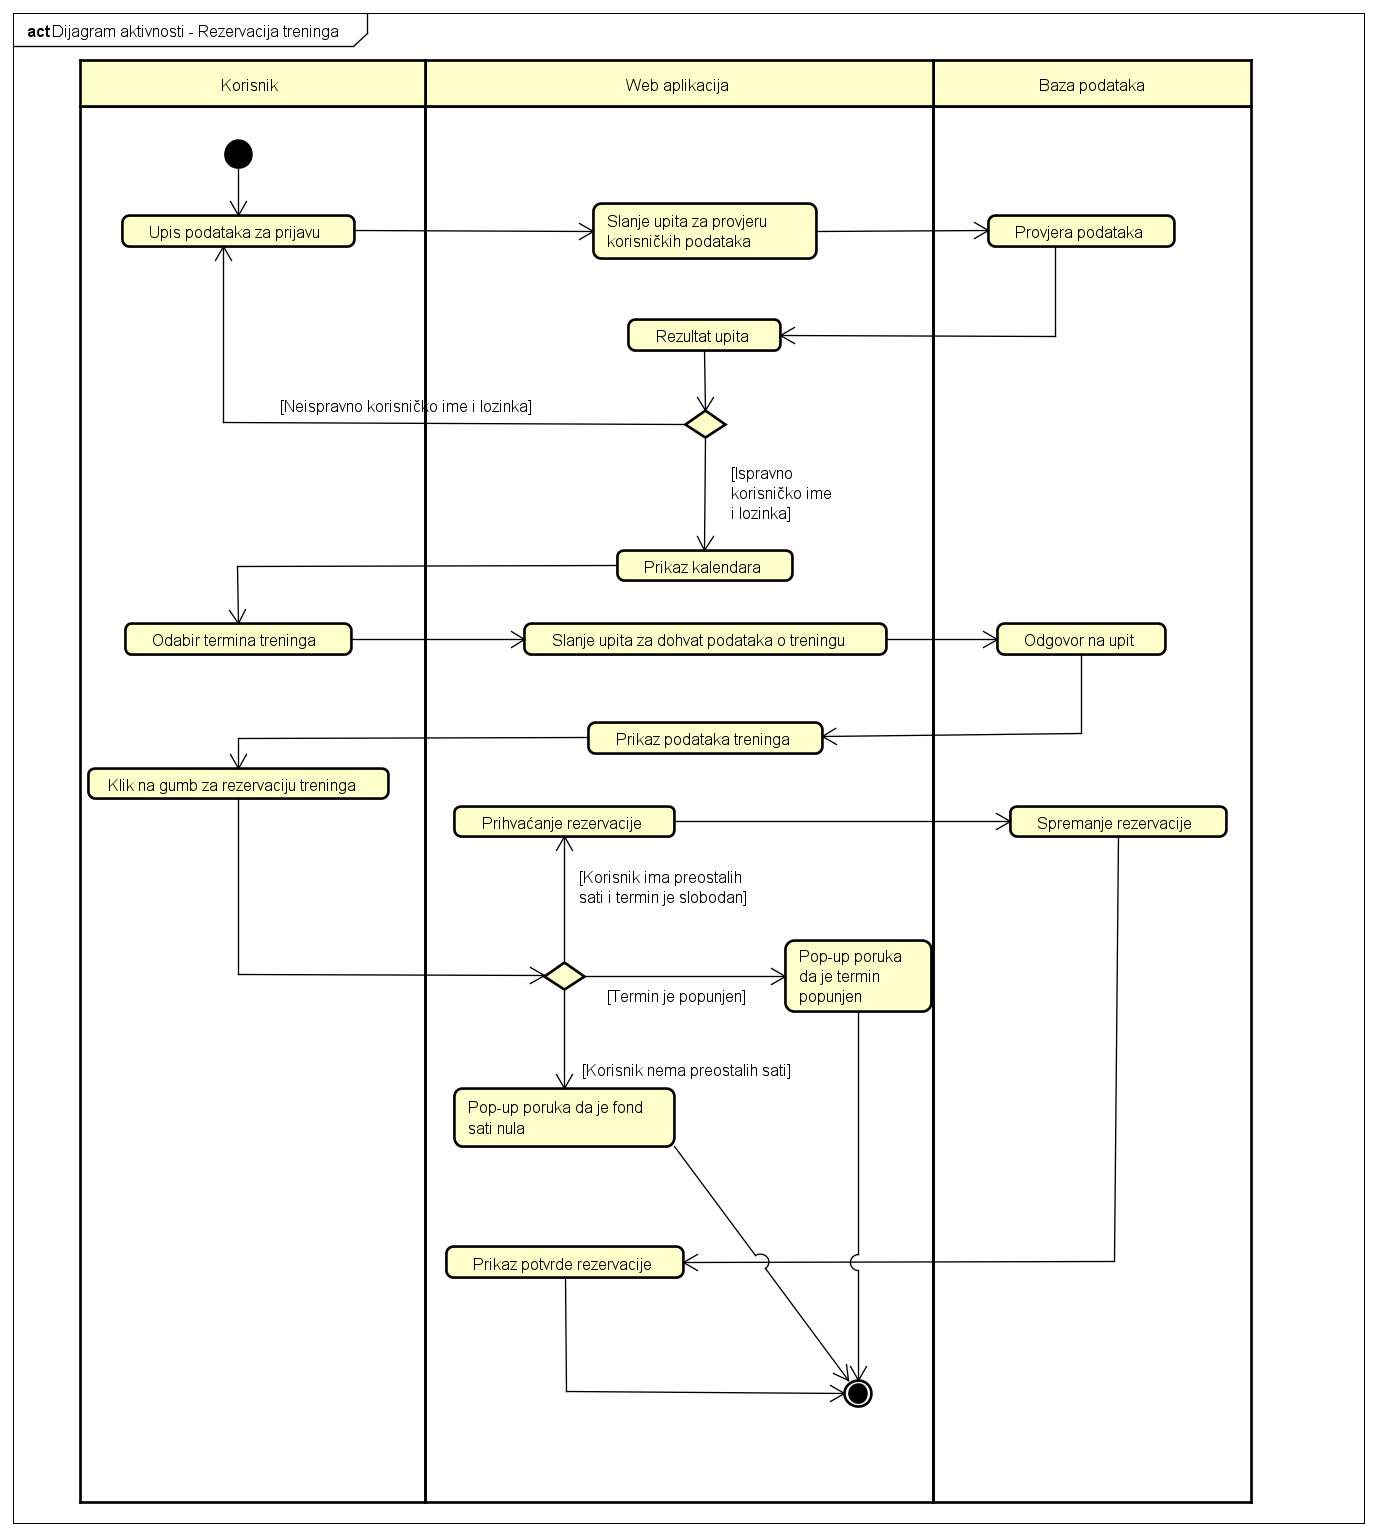
\includegraphics[scale=0.35]{dijagrami/Dijagram aktivnosti - Rezervacija treninga.png} %veličina slike u odnosu na originalnu datoteku i pozicija slike
			 	\centering
			 	\caption{Dijagram aktivnosti - Rezervacija treninga}
			 	\label{fig:dijagramaktivnosti}
			 \end{figure}
			
			\eject
		\section{Dijagram komponenti}
		
		{Dijagram komponenti statički je UML dijagram. Slika \ref {fig:dijagramkomponenti} opisuje organizaciju i međuovisnost
			komponenti, interne strukture i odnose prema okolini. Razlikujemo dva različita sučelja. Preko sučelja za dohvat HTML, CSS i JS datoteka poslužuju se datoteke koje pripadaju klijentskom dijelu aplikacije. App.js komponenta je koja na
			upit s url određuje koja će se datoteka poslužiti na sučelje. Klijentski dio aplikacije se sastoji od niza JavaScript datoteka koje su sakupljene u komponentu Pages. Sve JavaScript datoteke ovise o React biblioteci iz
			koje dohvaćaju gotove komponente kao što su gumbi i forme. Preko sučelja za dohvat JSON podataka pristupa se REST API komponenti. REST API poslužuje podatke koji pripadaju poslužiteljskom dijelu aplikacije. Repository komponenta
			služi za dohvaćanje tablica iz baze podataka pomoću SQL upita. React-view komponenta preko dostupnih sučelja komunicira s aplikacijom te ovisno o akcijama korisnika osvježava prikaz i dohvaća nove podatke.}
		
			\begin{figure}[H]
				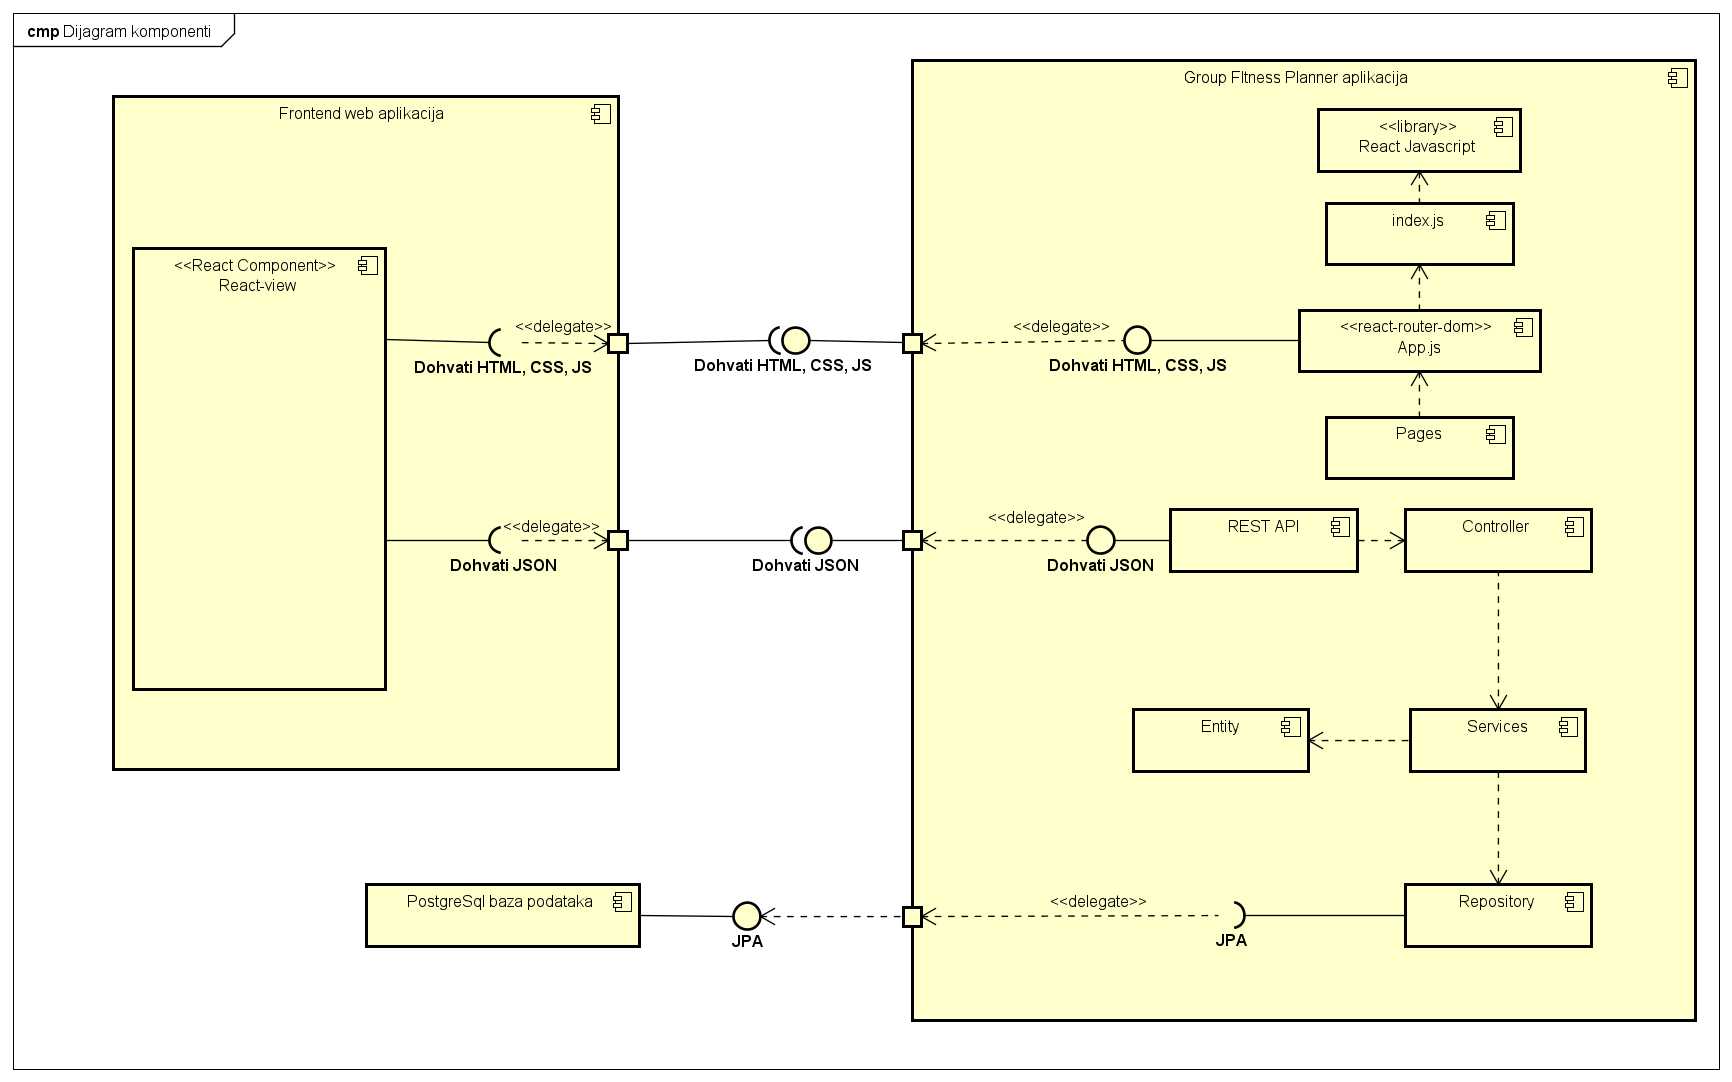
\includegraphics[scale=0.35]{dijagrami/Dijagram komponenti.png} %veličina slike u odnosu na originalnu datoteku i pozicija slike
				\centering
				\caption{Dijagram komponenti}
				\label{fig:dijagramkomponenti}
			\end{figure}
